\begin{figure}
	\centering
	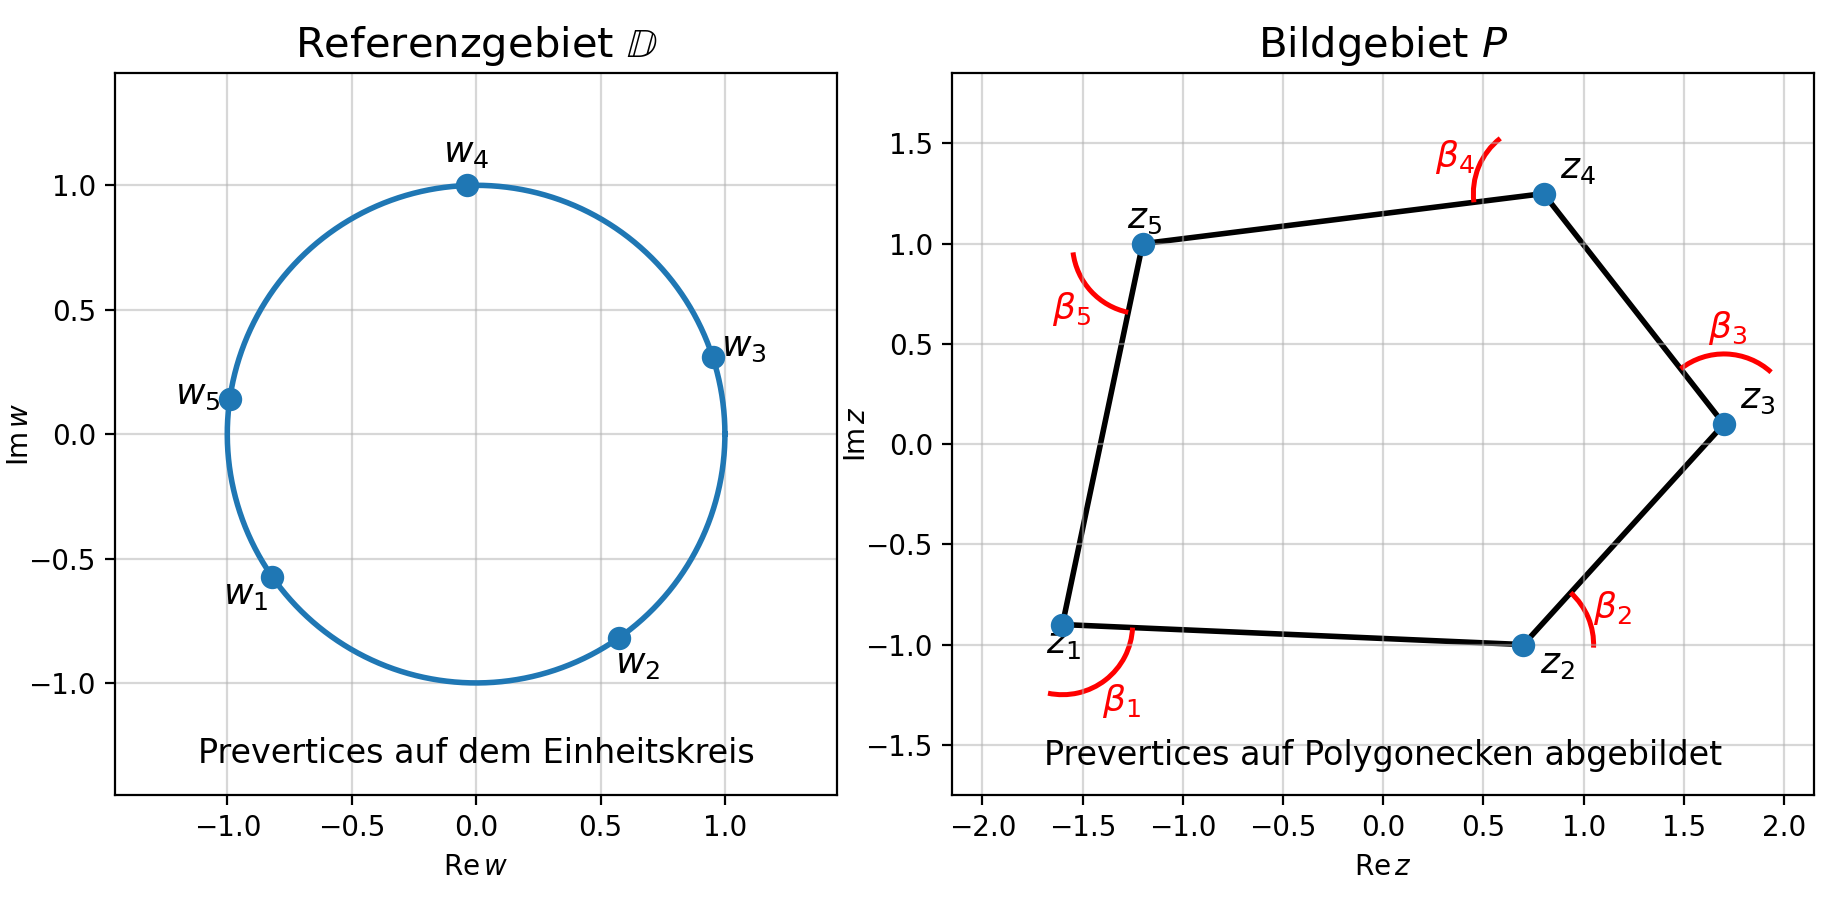
\includegraphics[width=\textwidth]{papers/elektro/grafik/SC_trafo_erklaerung.png}
	\caption{Zuordnung zwischen dem Einheitskreis und dem Polygon bei der Schwarz-Christoffel-Transformation.
        Links liegen die Prevertices $w_k$ auf dem Rand des Einheitskreises.
        Durch die Abbildung $f$ werden sie auf die entsprechenden Ecken $z_k$ des Polygons rechts abgebildet.
        Die Winkel $\alpha_k$ bezeichnen die Innenwinkel des Polygons.}
	\label{elektro:figure:SchwarzChristoffel_erklaerung}
\end{figure}
